\documentclass[final]{baposter}

%
% Para compilar: latex  poster2010.tex (dos veces)
%                dvips  poster2010.dvi
%                ps2pdf poster2010.ps 
%
%                (no funciona con pdflatex ni con dvipdfm!!!)
%

\usepackage{times}
\usepackage{tikz}
\usepackage{calc}
\usepackage{graphicx}
\usepackage{amsmath}
\usepackage{amssymb}
\usepackage{relsize}
\usepackage{multirow}
\usepackage{bm}

\usepackage{graphicx}
\usepackage{multicol}

\usepackage{pgfbaselayers}
\pgfdeclarelayer{background}
\pgfdeclarelayer{foreground}
\pgfsetlayers{background,main,foreground}

\usepackage{helvet}
%\usepackage{bookman}
\usepackage{palatino}

\newcommand{\captionfont}{\footnotesize}

\selectcolormodel{cmyk}

%%%%%%%%%%%%%%%%%%%%%%%%%%%%%%%%%%%%%%%%%%%%%%%%%%%%%%%%%%%%%%%%%%%%%%%%%%%%%%%%
%%%% Some math symbols used in the text
%%%%%%%%%%%%%%%%%%%%%%%%%%%%%%%%%%%%%%%%%%%%%%%%%%%%%%%%%%%%%%%%%%%%%%%%%%%%%%%%
% Format 
\newcommand{\Matrix}[1]{\begin{bmatrix} #1 \end{bmatrix}}
\newcommand{\Vector}[1]{\Matrix{#1}}
\newcommand*{\SET}[1]  {\ensuremath{\mathcal{#1}}}
\newcommand*{\MAT}[1]  {\ensuremath{\mathbf{#1}}}
\newcommand*{\VEC}[1]  {\ensuremath{\bm{#1}}}
\newcommand*{\CONST}[1]{\ensuremath{\mathit{#1}}}
\newcommand*{\norm}[1]{\mathopen\| #1 \mathclose\|}% use instead of $\|x\|$
\newcommand*{\abs}[1]{\mathopen| #1 \mathclose|}% use instead of $\|x\|$
\newcommand*{\absLR}[1]{\left| #1 \right|}% use instead of $\|x\|$

\def\norm#1{\mathopen\| #1 \mathclose\|}% use instead of $\|x\|$
\newcommand{\normLR}[1]{\left\| #1 \right\|}% use instead of $\|x\|$

%%%%%%%%%%%%%%%%%%%%%%%%%%%%%%%%%%%%%%%%%%%%%%%%%%%%%%%%%%%%%%%%%%%%%%%%%%%%%%%%
% Multicol Settings
%%%%%%%%%%%%%%%%%%%%%%%%%%%%%%%%%%%%%%%%%%%%%%%%%%%%%%%%%%%%%%%%%%%%%%%%%%%%%%%%
\setlength{\columnsep}{0.7em}
\setlength{\columnseprule}{0mm}

%%%%%%%%%%%%%%%%%%%%%%%%%%%%%%%%%%%%%%%%%%%%%%%%%%%%%%%%%%%%%%%%%%%%%%%%%%%%%%%%
% Save space in lists. Use this after the opening of the list
%%%%%%%%%%%%%%%%%%%%%%%%%%%%%%%%%%%%%%%%%%%%%%%%%%%%%%%%%%%%%%%%%%%%%%%%%%%%%%%%
\newcommand{\compresslist}{%
\setlength{\itemsep}{1pt}%
\setlength{\parskip}{0pt}%
\setlength{\parsep}{0pt}%
}


%%%%%%%%%%%%%%%%%%%%%%%%%%%%%%%%%%%%%%%%%%%%%%%%%%%%%%%%%%%%%%%%%%%%%%%%%%%%%%
%%% Begin of Document
%%%%%%%%%%%%%%%%%%%%%%%%%%%%%%%%%%%%%%%%%%%%%%%%%%%%%%%%%%%%%%%%%%%%%%%%%%%%%%

\begin{document}

%%%%%%%%%%%%%%%%%%%%%%%%%%%%%%%%%%%%%%%%%%%%%%%%%%%%%%%%%%%%%%%%%%%%%%%%%%%%%%
%%% Here starts the poster
%%%---------------------------------------------------------------------------
%%% Format it to your taste with the options
%%%%%%%%%%%%%%%%%%%%%%%%%%%%%%%%%%%%%%%%%%%%%%%%%%%%%%%%%%%%%%%%%%%%%%%%%%%%%%
%\typeout{Poster Starts}
%\background{
%  \begin{tikzpicture}[remember picture,overlay]%
    %\draw (current page.north west)+(-2em,-0em) node[anchor=north west] {\hspace{-2em}\includegraphics[height=1.1\textheight]{silhouettes_background}};
%  \end{tikzpicture}%
%}

% definidos por Guillermo Frank
\definecolor{Blue}{cmyk}{1.,1.,0,0} 
\definecolor{BlueViolet}{cmyk}{0.86,0.91,0,0.04} 
\definecolor{RoyalBlue}{cmyk}{1.,0.50,0,0}
\definecolor{SkyBlue}{cmyk}{0.62,0,0.12,0} 
\definecolor{TealBlue}{cmyk}{0.86,0,0.34,0.02}
\definecolor{CornflowerBlue}{cmyk}{0.65,0.13,0,0} 
\definecolor{NavyBlue}{cmyk}{0.94,0.54,0,0}
\definecolor{MidnightBlue}{cmyk}{0.98,0.13,0,0.43}
%\definecolor{mylightblue}{cmyk}{0.1,0.1,0.1,0.0}
\definecolor{mylightblue}{cmyk}{0.0,0.0,0.0,0.0}
\definecolor{mydarkblue}{cmyk}{1.,1.,0,0.63}
\definecolor{mylightgray}{cmyk}{0.19,0.15,0.01,0.5}

\pagecolor{mylightblue}


\begin{poster}{
  % Show grid to help with alignment
  grid=no,
  % Column spacing
  colspacing=1em,
  % Color style
  bgColorOne=mylightblue,                        
  bgColorTwo=mylightblue,                        
  borderColor=mylightgray,
  headerColorOne=mydarkblue,
  headerColorTwo=mydarkblue,
  %headerColorOne=olive!85!cyan,
  %headerColorTwo=olive!85!cyan,
  headerFontColor=white,
  boxColorOne=mylightblue,
  boxColorTwo=mydarkblue,
  % Format of textbox
  textborder=roundedleft,
  % Format of text header
  eyecatcher=yes,
  headerborder=open,
  headerheight=0.08\textheight,
  headershape=roundedright,
  headershade=plain,
  headerfont=\Large\textsf, %Sans Serif
  boxshade=plain,
  %background=shade-tb,
  background=plain,
  linewidth=2pt
  }
  % Eye Catcher
  {\begin{minipage}{10em}
    \vspace{7mm}
    \hfill
    
\includegraphics[height=6.5em]{logo_fcen}
    \vspace{5mm}
    %\includegraphics[height=5.5em]{logo}
  \end{minipage}} % No eye catcher for this poster. If an eye catcher is present, the title is centered between eye-catcher and logo.
  % Title
  {\sf %Sans Serif
  %\bf% Serif
  \textcolor{mydarkblue}{Self-propelled particles: evacuation through two doors \\}
\vspace{3mm}
\textcolor{mydarkblue}{\Large Ignacio Sticco, Guillermo Frank  \& 
Claudio Dorso 
{\large(codorso\textcolor{orange!90!black}{@}df.uba.ar)} }}
% Abstract #300660, Poster Session 253 on Monday, 8/1/2011 beginning at 2:00 PM
  % Authors
  {\sf %Sans Serif
  % Serif
 % \textcolor{mydarkblue}{\\ \vspace{-3mm}\Large Guillermo Frank
%{\large(frank\textcolor{red}{@}ieee.org)} \& Claudio Dorso 
%{\large(codorso\textcolor{red}{@}df.uba.ar)} } \hspace{6.5em}\\
    %\LARGE Guillermo A. Frank$^\textsf{1}$ - Claudio O. Dorso} \hspace{7.5em}
    %\textcolor{mylightgray}{$^{\textsf{(1)}}\,$frank@ieee.org} \hspace{5.5em}
    %\textcolor{mydarkblue}{\LARGE Universidad de Buenos Aires, Argentina}
  }
  % University logo
  {{\begin{minipage}{7em}
    \vspace{4mm}
    \hfill
    
\includegraphics[height=5.5em]{uba3}
    %\includegraphics[height=5.5em]{logo}
  \end{minipage}}
  }

  %\tikzstyle{light shaded}=[top color=baposterBGtwo!30!white,bottom color=baposterBGone!30!white,shading=axis,shading angle=30]

  % Width of left inset image
     %\newlength{\leftimgwidth}
     %\setlength{\leftimgwidth}{0.78em+8.0em}

%%%%%%%%%%%%%%%%%%%%%%%%%%%%%%%%%%%%%%%%%%%%%%%%%%%%%%%%%%%%%%%%%%%%%%%%%%%%%%
%%% Now define the boxes that make up the poster
%%%---------------------------------------------------------------------------
%%% Each box has a name and can be placed absolutely or relatively.
%%% The only inconvenience is that you can only specify a relative position 
%%% towards an already declared box. So if you have a box attached to the 
%%% bottom, one to the top and a third one which should be in between, you 
%%% have to specify the top and bottom boxes before you specify the middle 
%%% box.
%%%%%%%%%%%%%%%%%%%%%%%%%%%%%%%%%%%%%%%%%%%%%%%%%%%%%%%%%%%%%%%%%%%%%%%%%%%%%%
    %
    % A coloured circle useful as a bullet with an adjustably strong filling
    %\newcommand{\colouredcircle}[1]{%
    %  \tikz{\useasboundingbox (-0.2em,-0.32em) rectangle(0.2em,0.32em);  
    % \draw[draw=black,fill=baposterBGone!80!black!#1!white,line width=0.03em] 
    % (0,0) circle(0.18em);}}

%%%%%%%%%%%%%%%%%%%%%%%%%%%%%%%%%%%%%%%%%%%%%%%%%%%%%%%%%%%%%%%%%%%%%%%%%%%%%%
\headerbox{Outline}{name=contribution,column=0,span=3,row=0}{
%%%%%%%%%%%%%%%%%%%%%%%%%%%%%%%%%%%%%%%%%%%%%%%%%%%%%%%%%%%%%%%%%%%%%%%%%%%%%%

\Large Our research examines the statistical behaviour of escaping pedestrians 
when two contiguous exits are available, but placed at different separation 
distances. We found that the evacuation time can be improved if the separation 
exceeds a threshold distance. This threshold distance is related to changes in 
the clogging dynamics close to the doors.  
 }


%%%%%%%%%%%%%%%%%%%%%%%%%%%%%%%%%%%%%%%%%%%%%%%%%%%%%%%%%%%%%%%%%%%%%%%%%%%%%%
  \headerbox{What's about}{name=model,column=0,below=contribution,span=1.5}{
%%%%%%%%%%%%%%%%%%%%%%%%%%%%%%%%%%%%%%%%%%%%%%%%%%%%%%%%%%%%%%%%%%%%%%%%%%%%%%

  {\hspace*{3mm}
 % {\begin{minipage}{\textwidth}
  \begin{tabular}{c@{}c}
  \begin{minipage}{0.45\textwidth}
    \vspace{5mm}

    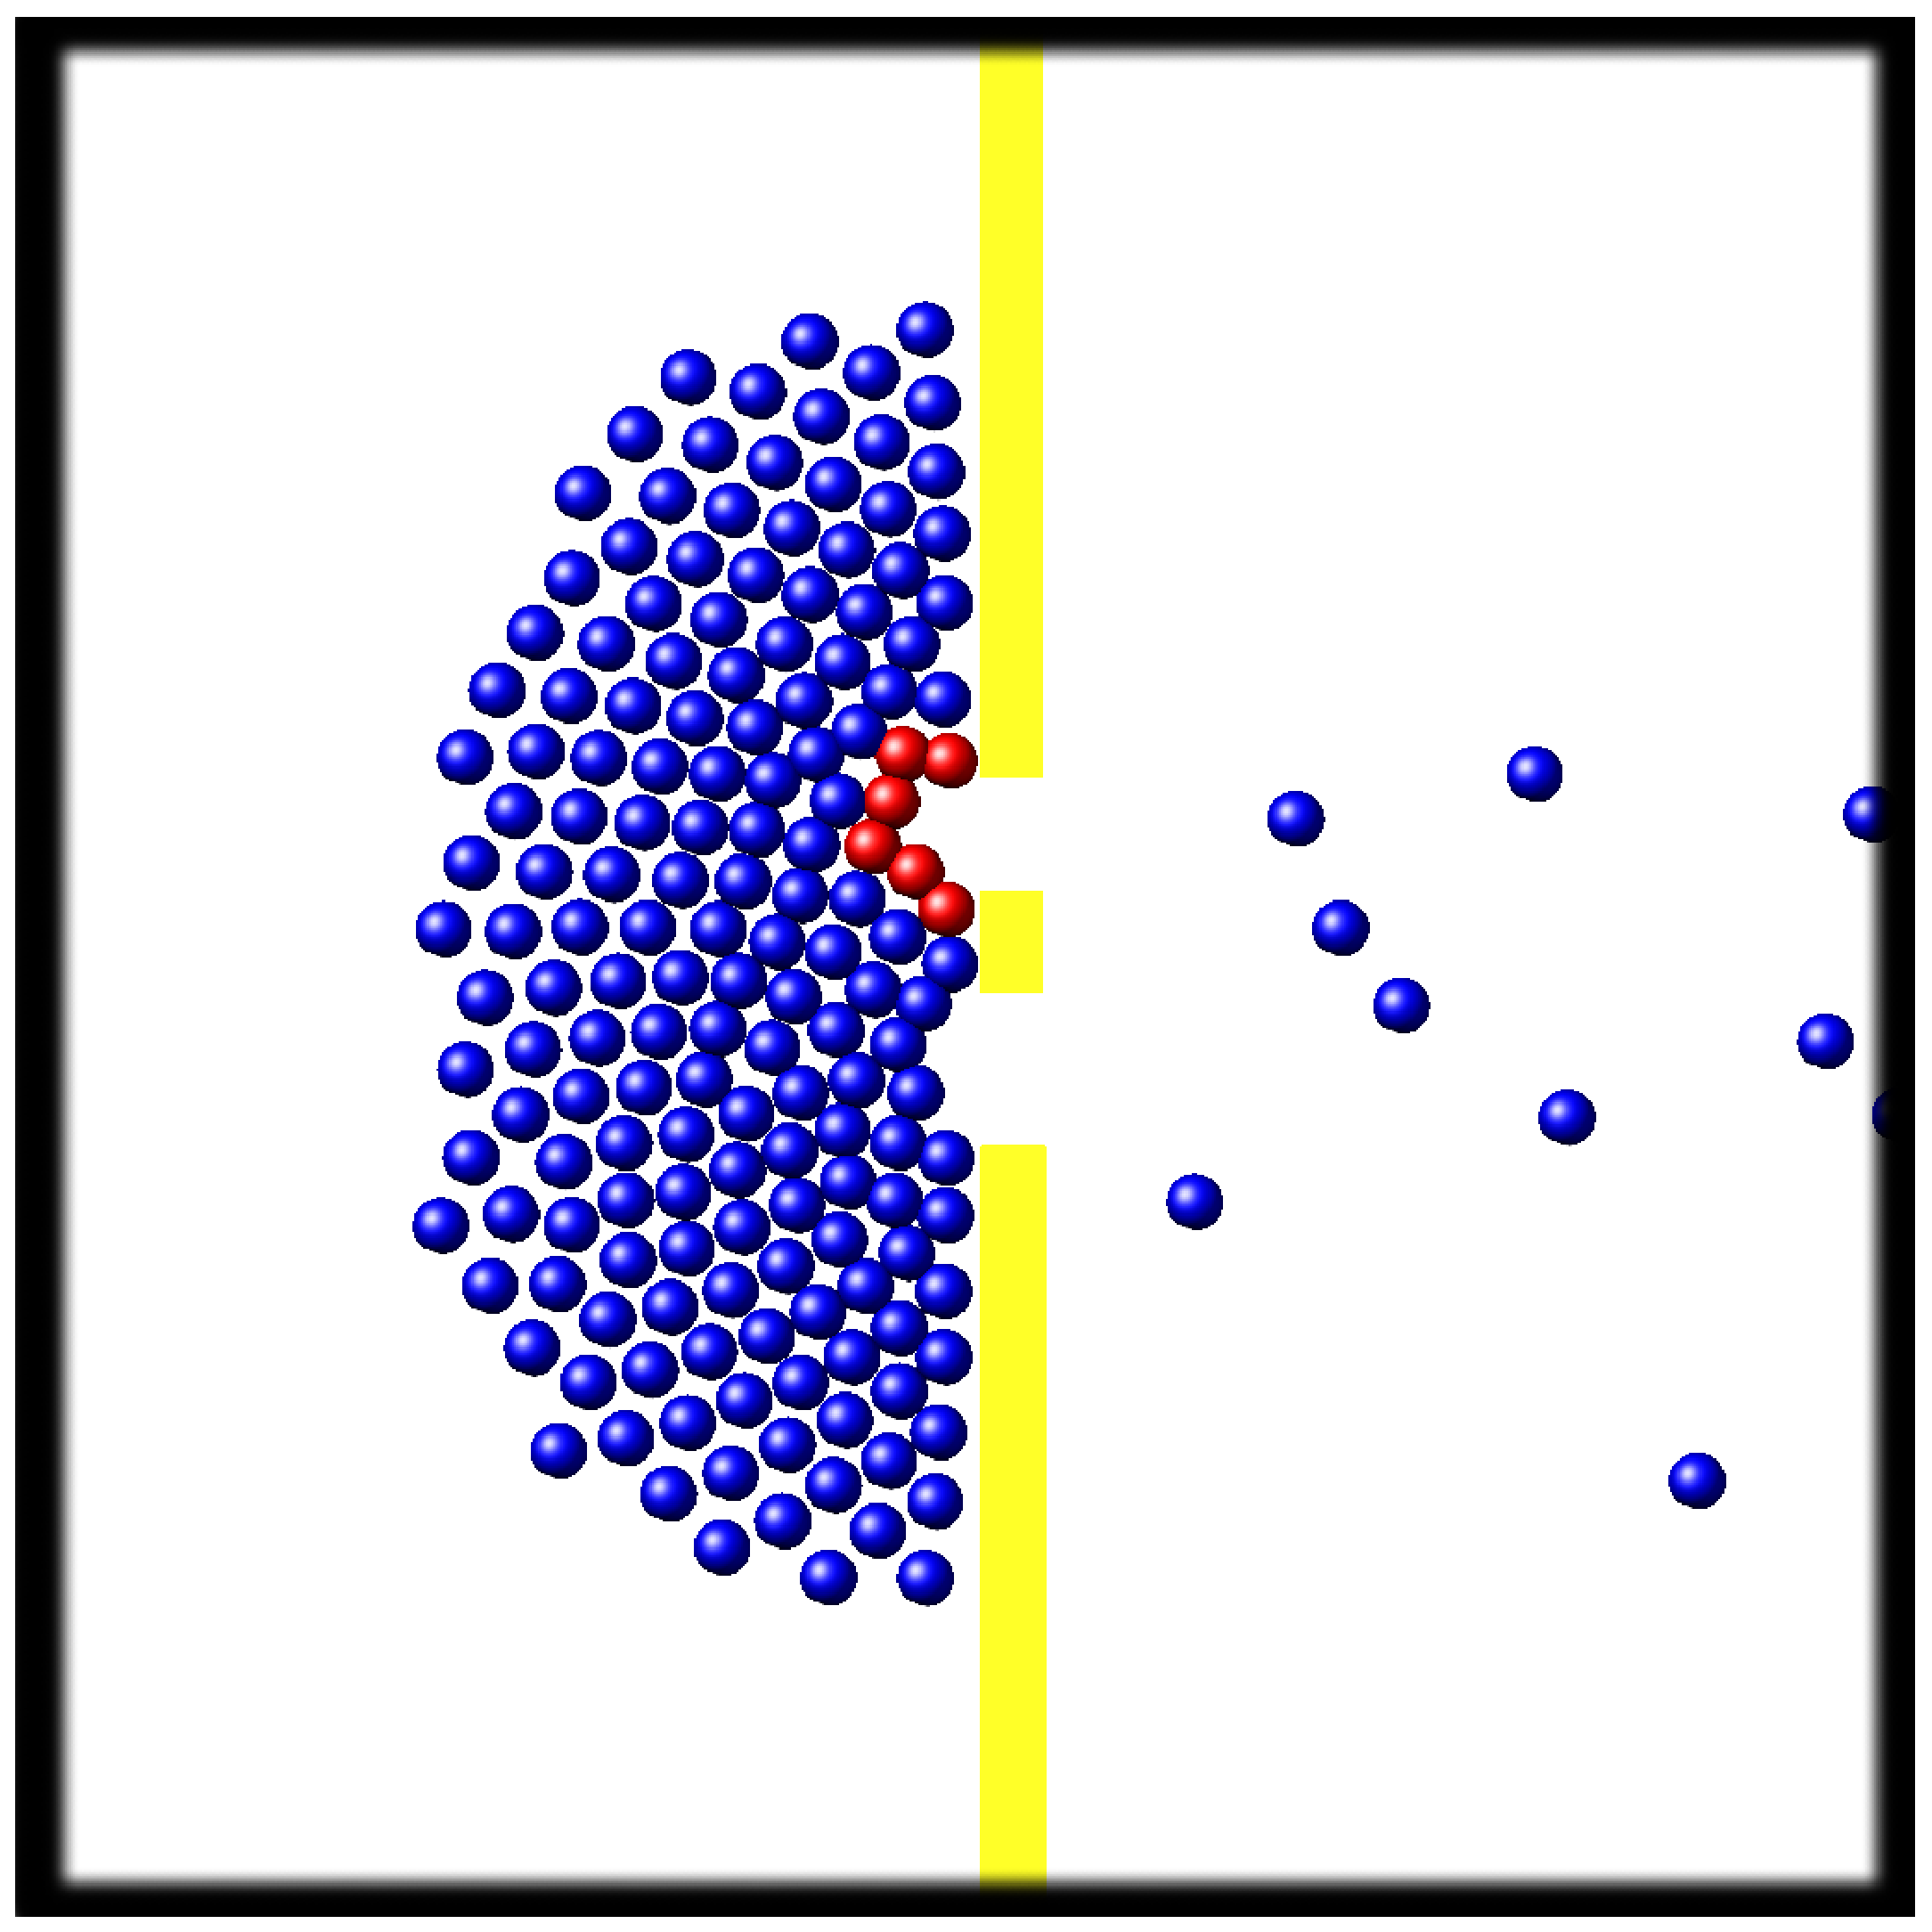
\includegraphics[scale=0.13]{./figures2/fig_poster_1.eps} \\  
    \vspace{5mm}
    
    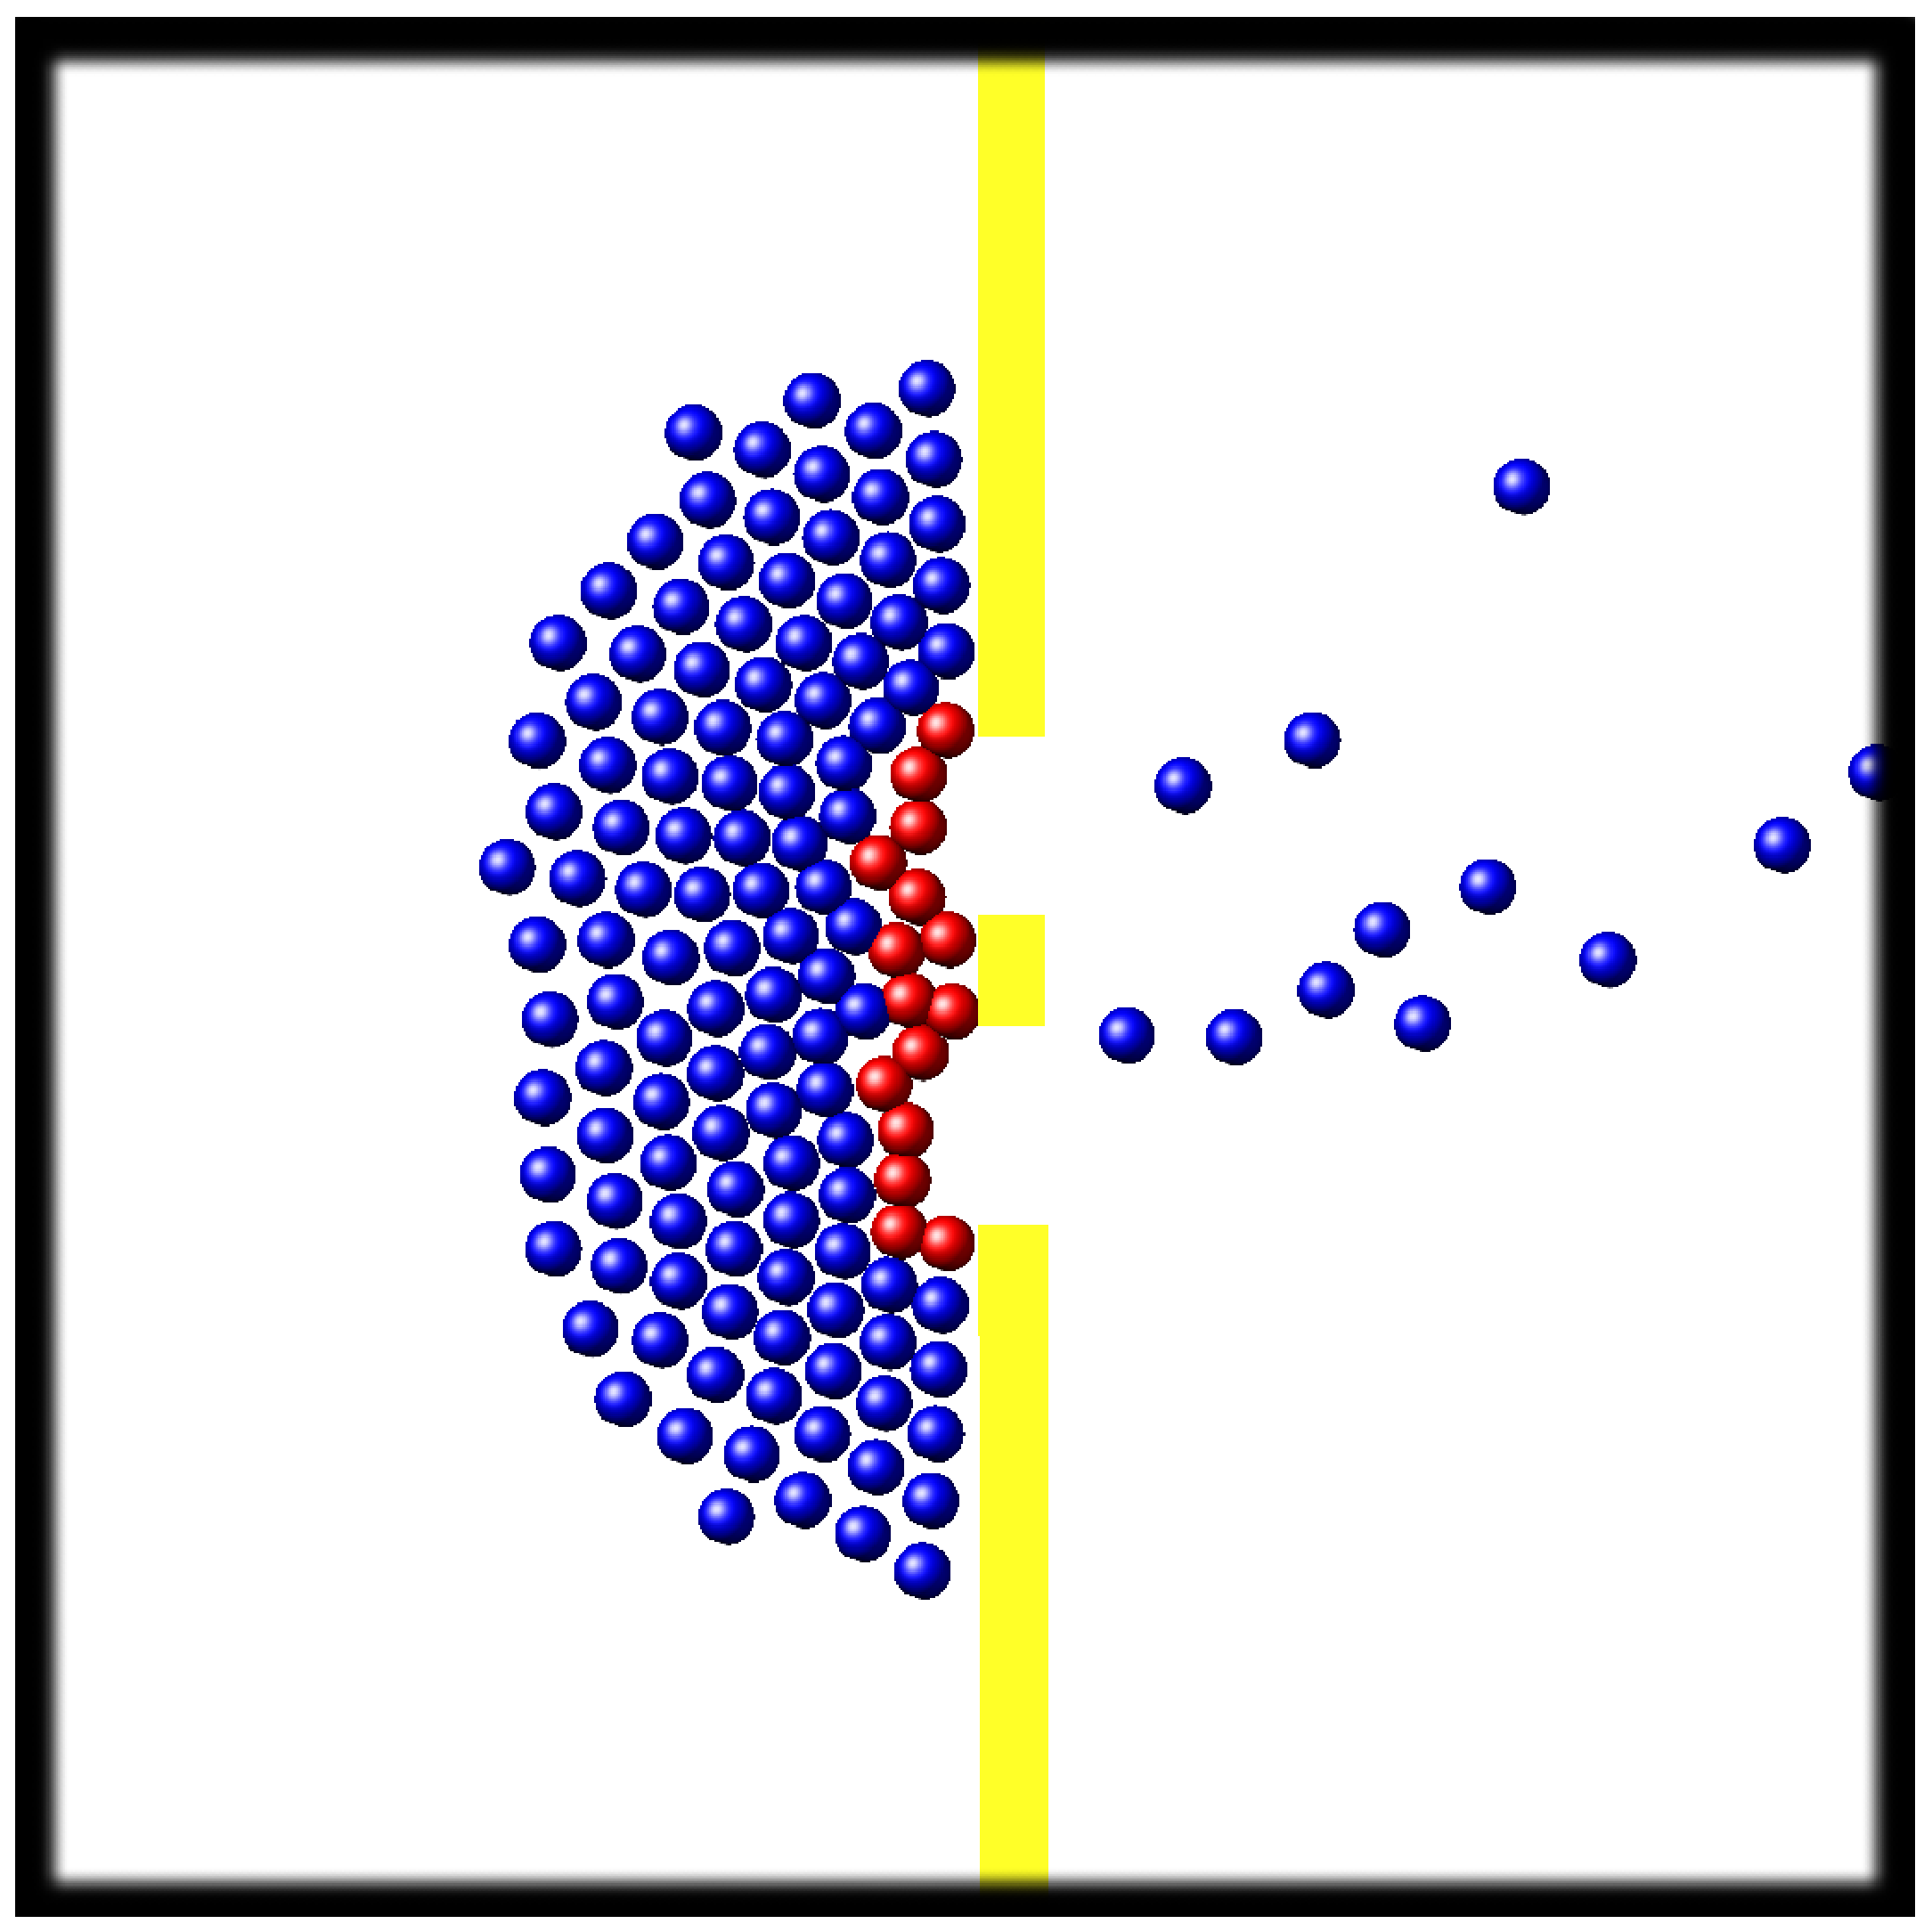
\includegraphics[scale=0.13]{./figures2/fig_poster_2.eps} 

  \end{minipage}
  & 
  
  \begin{minipage}{0.5\textwidth}
    \vspace{1mm}
   { \LARGE\begin{center}\textcolor{blue}{\bf\Large The Model (SFM):}\\
   \vspace{4mm}
$m\displaystyle\frac{d\mathbf{v}}{dt}=\mathbf{f}_d+\mathbf{f}
_s+\mathbf{f}_g$\\
\vspace{3mm}
\end{center}\Large

\begin{itemize}
\item $\mathbf{f}_d$ is the desire force
\item $\mathbf{f}_s$ is the social force
\item $\mathbf{f}_g$ is the sliding friction
\end{itemize}}

  \end{minipage}
    \end{tabular}  
  %\end{minipage}}
  }

  \vspace*{3mm}
  
  {\bf\textcolor{olive}{\Large \bf Individuals blocking the doors 
are coloured in red. The room size is 
20$\,$m$\times$20$\,$m (door width 1.2$\,$m). The 
desired velocity is $\mathbf{v_d=4\,}$m/s.}}\\ 


}


%%%%%%%%%%%%%%%%%%%%%%%%%%%%%%%%%%%%%%%%%%%%%%%%%%%%%%%%%%%%%%%%%%%%%%%%%%%%%%
  \headerbox{Pressure}{name=topics,column=0,span=1.5,below=model}{
%%%%%%%%%%%%%%%%%%%%%%%%%%%%%%%%%%%%%%%%%%%%%%%%%%%%%%%%%%%%%%%%%%%%%%%%%%%%%%

\Large
\vspace{2mm}
   \begin{minipage}{0.5\textwidth}
    \begin{center}
     Separation distance of 1.5~m.
     \end{center}
    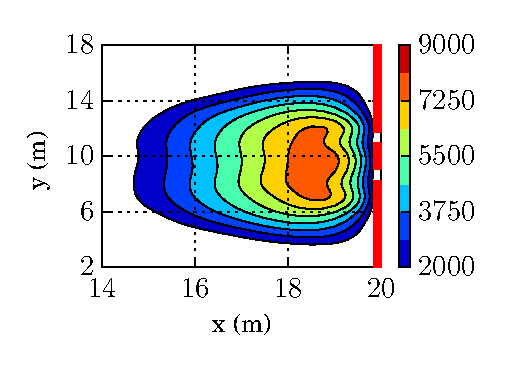
\includegraphics[scale=0.72]{./figures2/fig16_version0.eps}
    \end{minipage}
    %\hspace{0mm}
    \begin{minipage}{0.5\textwidth}
    \begin{center}
    Separation distance of 5~m.
    \end{center}
    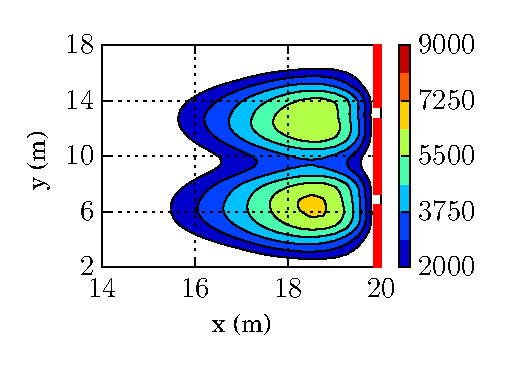
\includegraphics[scale=0.71]{./figures2/fig17_version0.eps}    
    \end{minipage}

\vspace{1.5mm}   
Fig~1. Mean pressures computed from 30 evacuation processes. 
$\,v_d=4\,$m/s. The scale bar on the right is expressed in N.m$^{-1}$ units. Red bars represent the walls.\\

\vspace{12mm}   
  

    
}


%%%%%%%%%%%%%%%%%%%%%%%%%%%%%%%%%%%%%%%%%%%%%%%%%%%%%%%%%%%%%%%%%%%%%%%%%%%%%%
\headerbox{Evacuation time}{name=results,below=contribution,column=1.5,span=1.5,row=0}{
%%%%%%%%%%%%%%%%%%%%%%%%%%%%%%%%%%%%%%%%%%%%%%%%%%%%%%%%%%%%%%%%%%%%%%%%%%%%%%


  {\hspace*{23mm}
 % {\begin{minipage}{\textwidth}
  \begin{tabular}{c@{}c}
  \begin{minipage}{0.45\textwidth}
    %\vspace{1mm}

    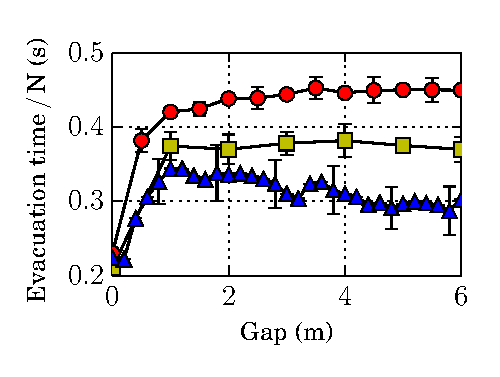
\includegraphics[scale=0.80]{./figures2/fig1_version0.eps} \\  
    %\vspace{0.1mm}   
    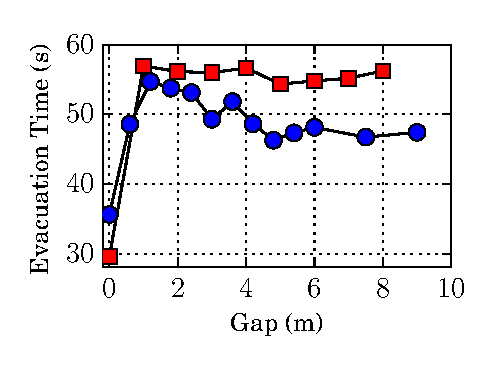
\includegraphics[scale=0.80]{./figures2/fig12_version0.eps} 

  \end{minipage}
  & 
  
 % \begin{minipage}{0.5\textwidth}
  %  \vspace{1mm}
    
	
  %\end{minipage}
    \end{tabular}  
  %\end{minipage}}
  }

  \vspace*{3mm}
  
  {\Large Fig~2. Mean evacuation time for 225 pedestrians computed from 30 evacuation processes.~\textcolor{olive}{(Up)} {\color{blue} $\blacktriangle$} corresponds to 225 individuales, rectangle \fill[yellow!75!green] (0,0) rectangle (0.28,0.28); \hspace{2.5mm}  corresponds to 584 individuals and \tikz\draw[red,fill=red] (0,0) circle (.5ex); corresponds to 960 individuals ($v_d=4\,$m/s).~\textcolor{olive}{(Down)} \tikz\draw[blue,fill=blue] (0,0) circle (.5ex); 225 individuals and $v_d=4\,$m/s.~\fill[red!40!red] (0,0) rectangle (0.28,0.28); \hspace{2.5mm}  225 individuals and $v_d=8\,$m/s.}\\  


}




%%%%%%%%%%%%%%%%%%%%%%%%%%%%%%%%%%%%%%%%%%%%%%%%%%%%%%%%%%%%%%%%%%%%%%%%%%%%%%
  
\headerbox{Conclusions}{name=questions,column=1.5,span=1.5,below=results} {
%%%%%%%%%%%%%%%%%%%%%%%%%%%%%%%%%%%%%%%%%%%%%%%%%%%%%%%%%%%%%%%%%%%%%%%%%%%%%%

\Large 

\begin{itemize}
\item[\textcolor{blue}{\checkmark}] Short separation distances (Gap $\simeq1.2$ m) worsen the evacuation performance for all the explored situations, 
while larger distances (Gap $>1.2\,$m) enhances the evacuation time for 
relatively small crowds and moderate anxiety levels.
\item[\textcolor{blue}{\checkmark}]As the separation distance approaches 
$1.2\,$m (from the null distance), the probability of having blocking 
structures around each door raises, resembling the situation of two independent 
doors.
\item[\textcolor{blue}{\checkmark}] Increasing the crowd size ($N$) or the 
pedestrian's anxiety level ($v_d$) slows down the evacuation. Both magnitudes 
raise the pressure acting on the pedestrians.
\end{itemize}

  }%

%%%%%%%%%%%%%%%%%%%%%%%%%%%%%%%%%%%%%%%%%%%%%%%%%%%%%%%%%%%%%%%%%%%%%%%%%%%%%%
 
\headerbox{Acknowledgements}{name=Acknowledgements,column=0,
span=3,above=bottom,below=topics}{
%%%%%%%%%%%%%%%%%%%%%%%%%%%%%%%%%%%%%%%%%%%%%%%%%%%%%%%%%%%%%%%%%%%%%%%%%%%%%%

\large  

%\vspace{0.5mm}

C.O. Dorso is a main researcher of the National Scientific Technical Research Council (CONICET- Argentina) and full professor FCEN-UBA. G. Frank is an  assistant researcher of the CONICET. I. Sticco has degree in Physics. 
  }%

\end{poster}%
%



\end{document}
